
%%%%%%%%%%%%%%%%%%%%%%%%%%%%%%%%%%%%%%%%%%%%%%%%%%%%%%%%%%%%%%%%%%%%
\section{Installation, Integration and Commissioning (David Newbold \& Alec Habig)}
\label{sec:fdsp-daq-install}

\metainfo{2 Pages}

%%%%%%%%%%%%%%%%%%%%%%%%%%%%%%%%%%%%
\subsection{Installation}
\label{sec:fdsp-daq-install-transport}

The DAQ will be installed in the server room part of the control room
area of the CUC as diagrammed in Fig.~\ref{fig:daq-install-controlroom},
starting as soon as the consortium has beneficial occupancy of this
space.  Fiber will be run from both the detectors' WIBs and the surface,
installed by the CF group.  This starting point is currently projected
to be eighteen months before APAs can be installed in cryostats,
allowing time for the DAQ to be ready to be used for APA testing and
commissioning.

\SI{500}{kVA} of power and cooling will be available to run the
computers in this room.  12 standard \SI{19}{in} server racks of DAQ
space per module were initially allocated, with two more each for
facilities and CISC.  This room design has more floor space than
initially proposed, potentially creating more space for racks or a
workbench: optimization of space vs. power consumption are being worked
out.  The racks will be water cooled. To allow expanded headroom for
initial testing, development, and commissioning throughput, the full
complement of DAQ hardware will be installed right away: even though
only the first two modules will need to use it.

\begin{dunefigure}[CUC Control Room Layout]{fig:daq-install-controlroom}
  {Floor plan for the DAQ and control room space in the CUC.  The ``Data
    Room'' has space for at least 52 racks of servers and routers.
    Fiber from the WIBs in the detector caverns will enter in the upper
    right of this room, terminate in a breakout panel, and be
    distributed to the RCEs in these racks, then to FELIX servers (also
    in this room) as outlined in
    Fig.~\ref{fig:daq-readout-buffering-baseline}.  Fibers to the
    surface will enter this room from the lower left.}
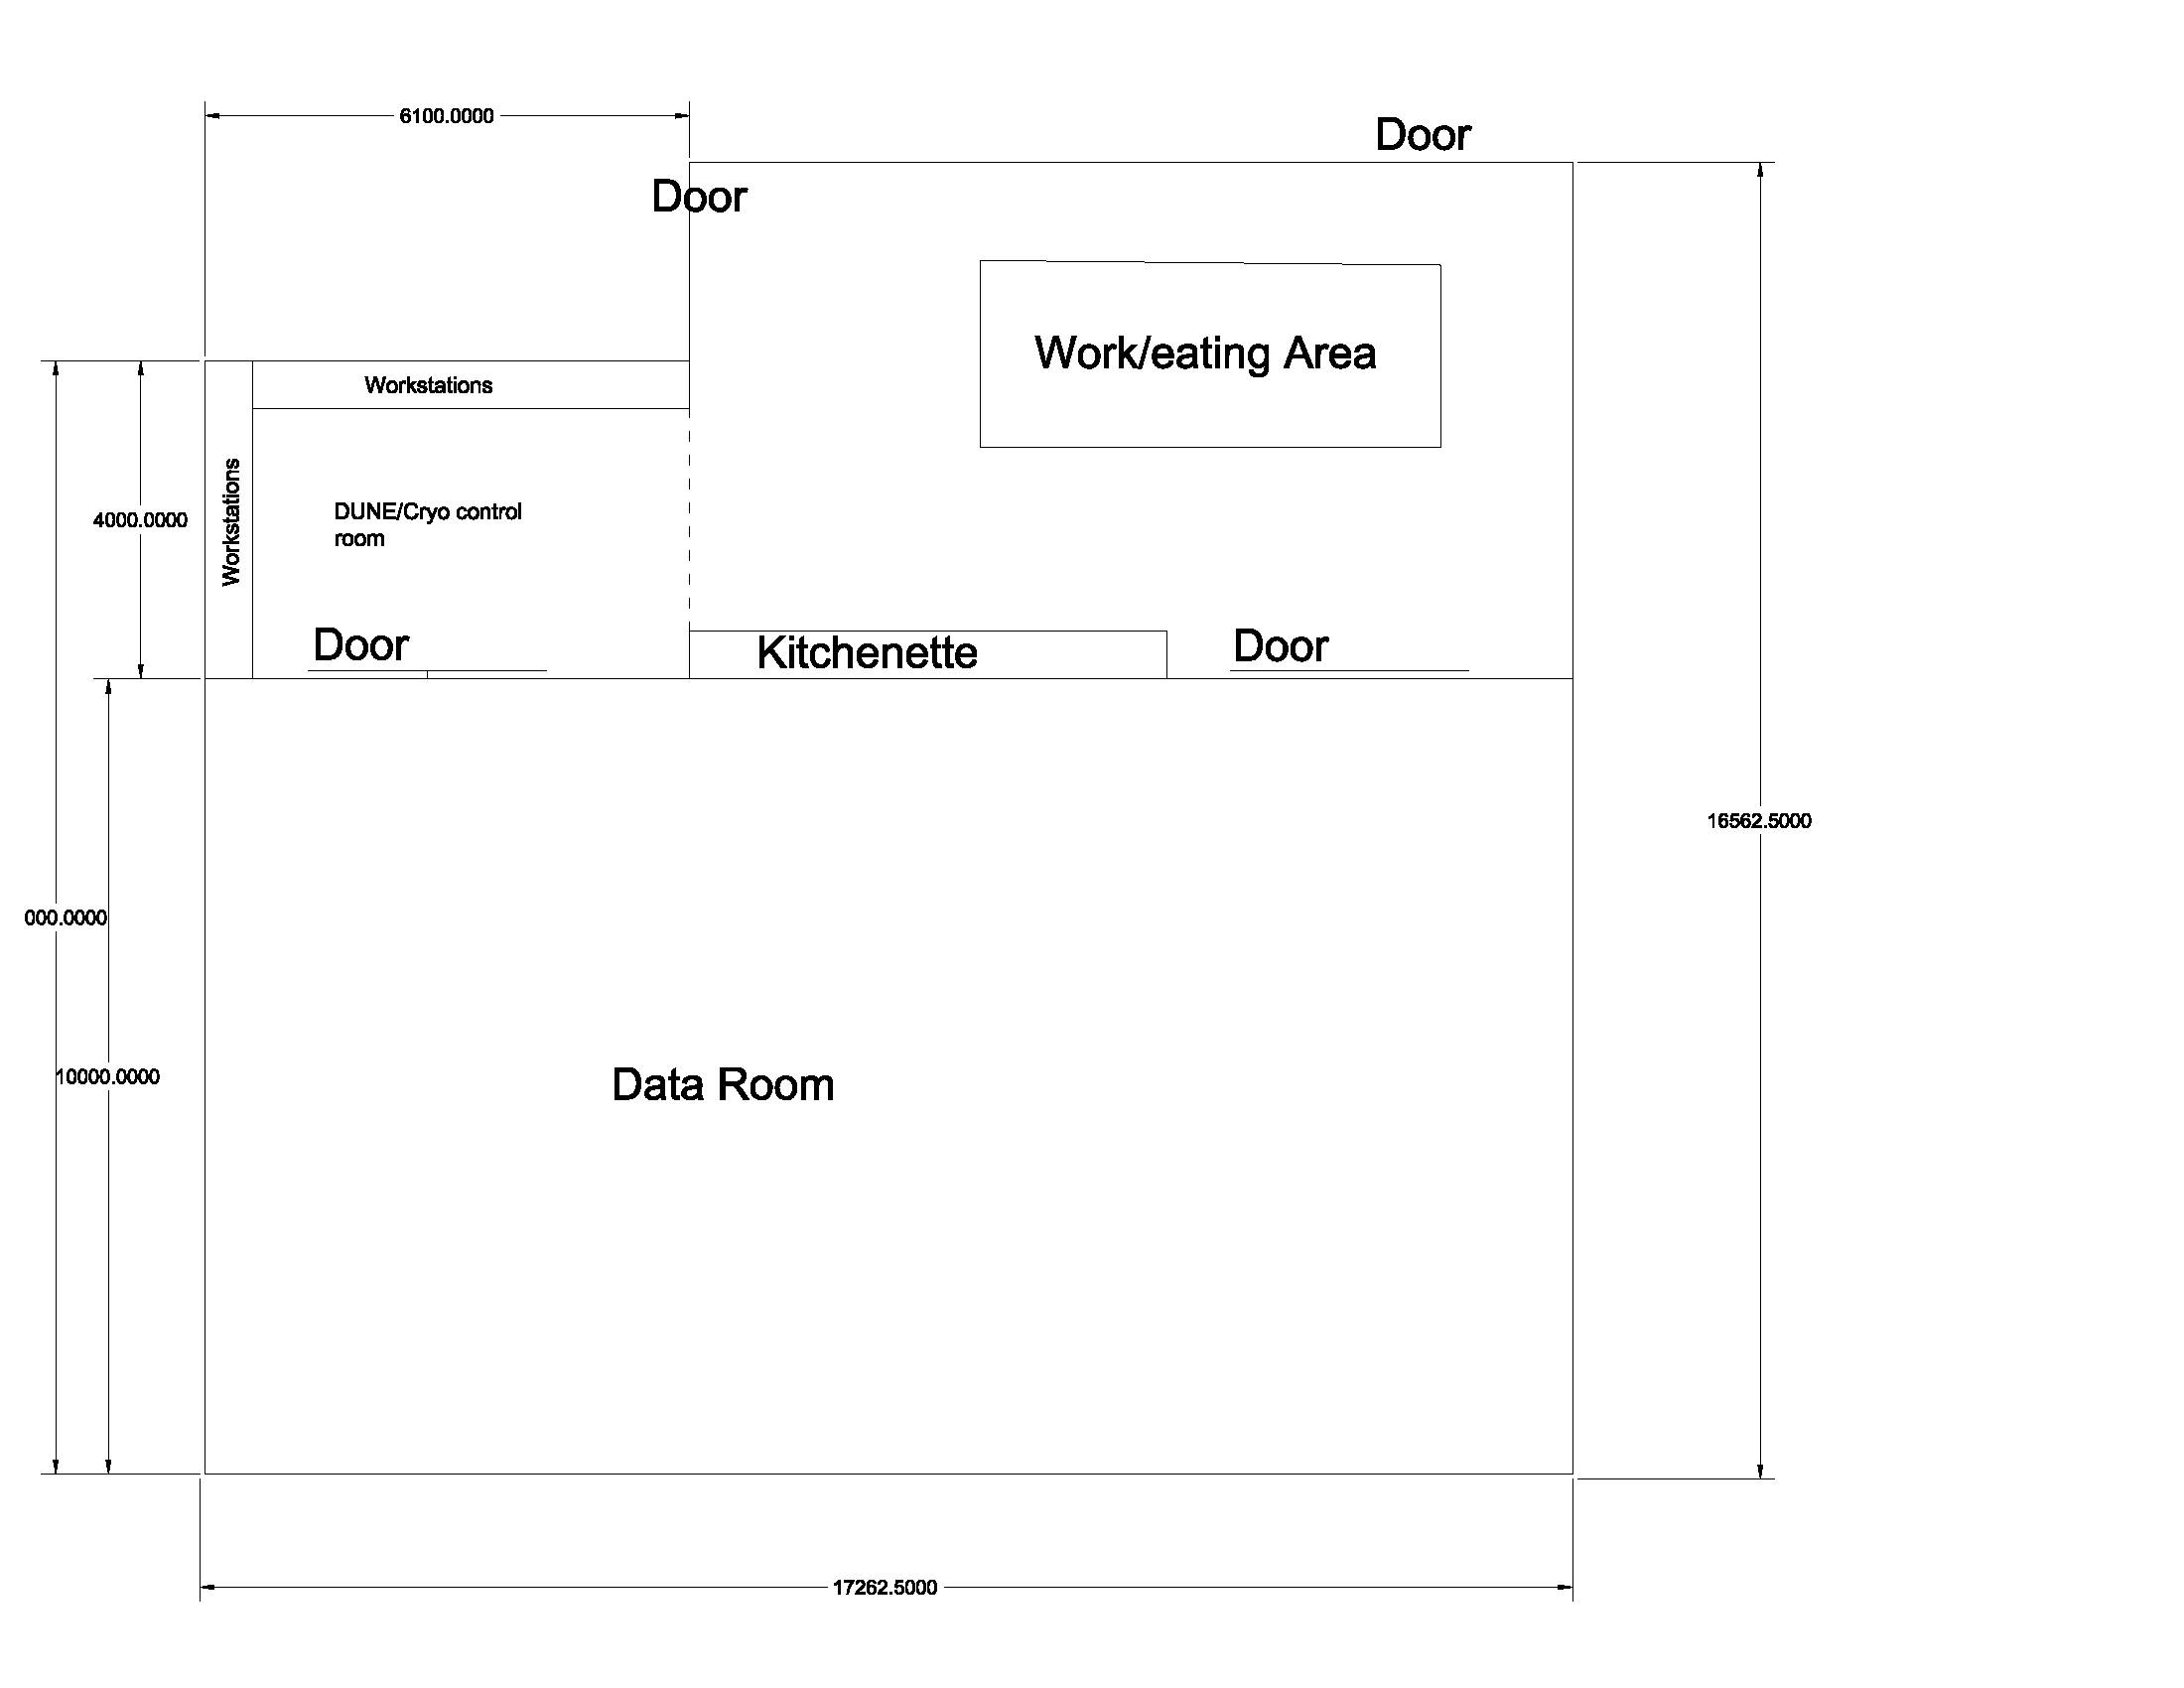
\includegraphics[width=0.8\textwidth]{ControlRoom-v2.png}
\end{dunefigure}

This room will be similar to any server room at a university or national
lab in terms of need for cleanliness, ventilation, fire protection, drop
flooring, and access.  Networking infrastructure and fiber breakout will
take up some of the rack space, but not very much of the power budget.
 Power to individual machines will need to be controlled remotely via
power distribution units, as a goal is to minimize DAQ workers
underground if there is work which can be done from the surface or
remotely instead.  Some UPS capacity will be needed to allow for an
orderly shutdown of computers, but only networking equipment will need
longer duration backup power, to enable remote recovery from short-term
power failures.  

%%%%%%%%%%%%%%%%%%%%%%%%%%%%%%%%%%%%
\subsection{Integration with TPC/PD Electronics}
\label{sec:fdsp-daq-install-transport}


%%%%%%%%%%%%%%%%%%%%%%%%%%%%%%%%%%%
\subsection{Commissioning}
\label{sec:fdsp-daq-commissioning}

\fixme{Commissioning of the DAQ or using the DAQ to commission the APAs?}

% %%%%%%%%%%%%%%%%%%%%%%%%%%%%%%%%%%%
% \subsection{Calibration?}
% \label{sec:fdsp-daq-install-calib}
%
% \fixme{Not needed ?}


% %%%%%%%%%%%%%%%%%%%%%%%%%%%%%%%%%%%%%%%%%%%%%%%%%%%%%%%%%%%%%%%%%%%%
% \section{Quality Control}
% \label{sec:fdsp-daq-qc}
%
% %%%%%%%%%%%%%%%%%%%%%%%%%%%%%%%%%%%%
% \subsection{Protection and Assembly (Local)}
% \label{sec:fdsp-daq-qc-local}
%
%
% %%%%%%%%%%%%%%%%%%%%%%%%%%%%%%%%%%%
% \subsection{Post-factory Installation (Remote)}
% \label{sec:fdsp-daq-qc-remote}
%
%

